% !TEX root = ../paper.tex
\section{Experiments} \label{sec:experiment}
% Intro
In order to compare  different techniques to each other we conducted an experiment in which each participant would perform the techniques in a controlled environment.
There are two parts to this experiment because after we finished the first experiment we realized that before we could say anything about accuracy in pixels we would have to design an experiment that required people to aim at a precise point and tell the participants to be as precise as they could.
Not having told our first 51 participants to aim and be precise we did the experiment again, adding a precise point to aim after for each target.
The first  experiment will be referred to as \target, and the second will be referred to as \accuracy.

\subsection{Implementation}

The four interaction techniques were implemented in a test application were the main goal was to correctly put shapes onto the screen from the smart phone or pull them away from the screen and put them on the phone.
The shapes would represent data, and two shapes(square and circle) were used in order to simulate the effect of choice of data. 

A grid system was implemented, were each target could be located in a particular grid cell.
The grid had two different sizes.
One was a large cell system, which had $5\times10$ cells, and each cell measured 61 pixels (7.3 cm) on each side.
The other was a small cell system, with $10\times20$ cells, each cell measuring 122 pixels (14.6 cm)  on each side. 

Shapes would appear in the cells, filling 80\% of it. 
These shapes would appear according to a predetermined series of locations, so that we could ensure that each target had an equal distribution of distances between them. 
For the user, the sequence would appear as random. 
These shapes would represent targets which the user had to hit.
A blue circle was used to represent were the user is pointing on the screen
This is were the user would ``hit'' whenever he performed an attempt with a given technique.

\begin{figure}[H]
	\begin{minipage}[c]{.12\columnwidth}
	\centering
	\subfloat[]{\includegraphics[width = 1\columnwidth]{images/target.pdf}\label{fig:target}}\\
	\subfloat[]{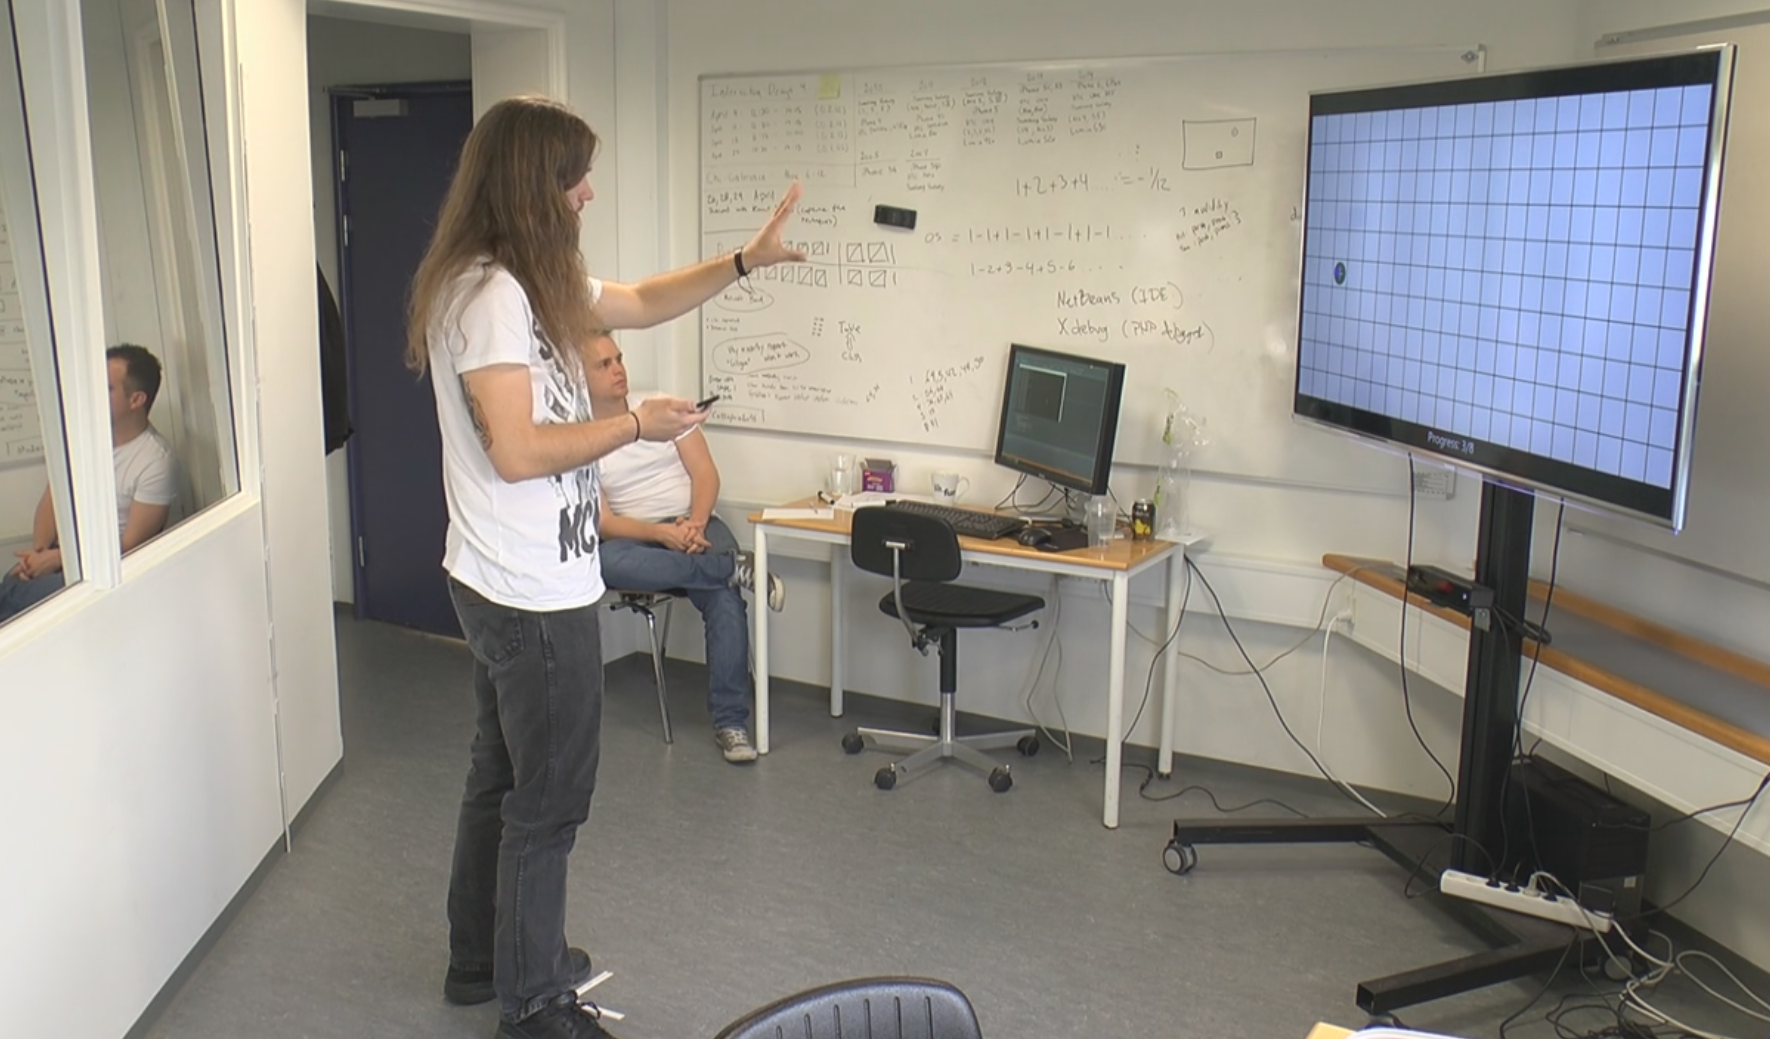
\includegraphics[width = 1\columnwidth]{images/accuracy.pdf}\label{fig:accuracy}}
	\end{minipage}%
	\hspace{0.01\columnwidth}
	\begin{minipage}[c]{.88\columnwidth}
	\centering
	\subfloat[\push]{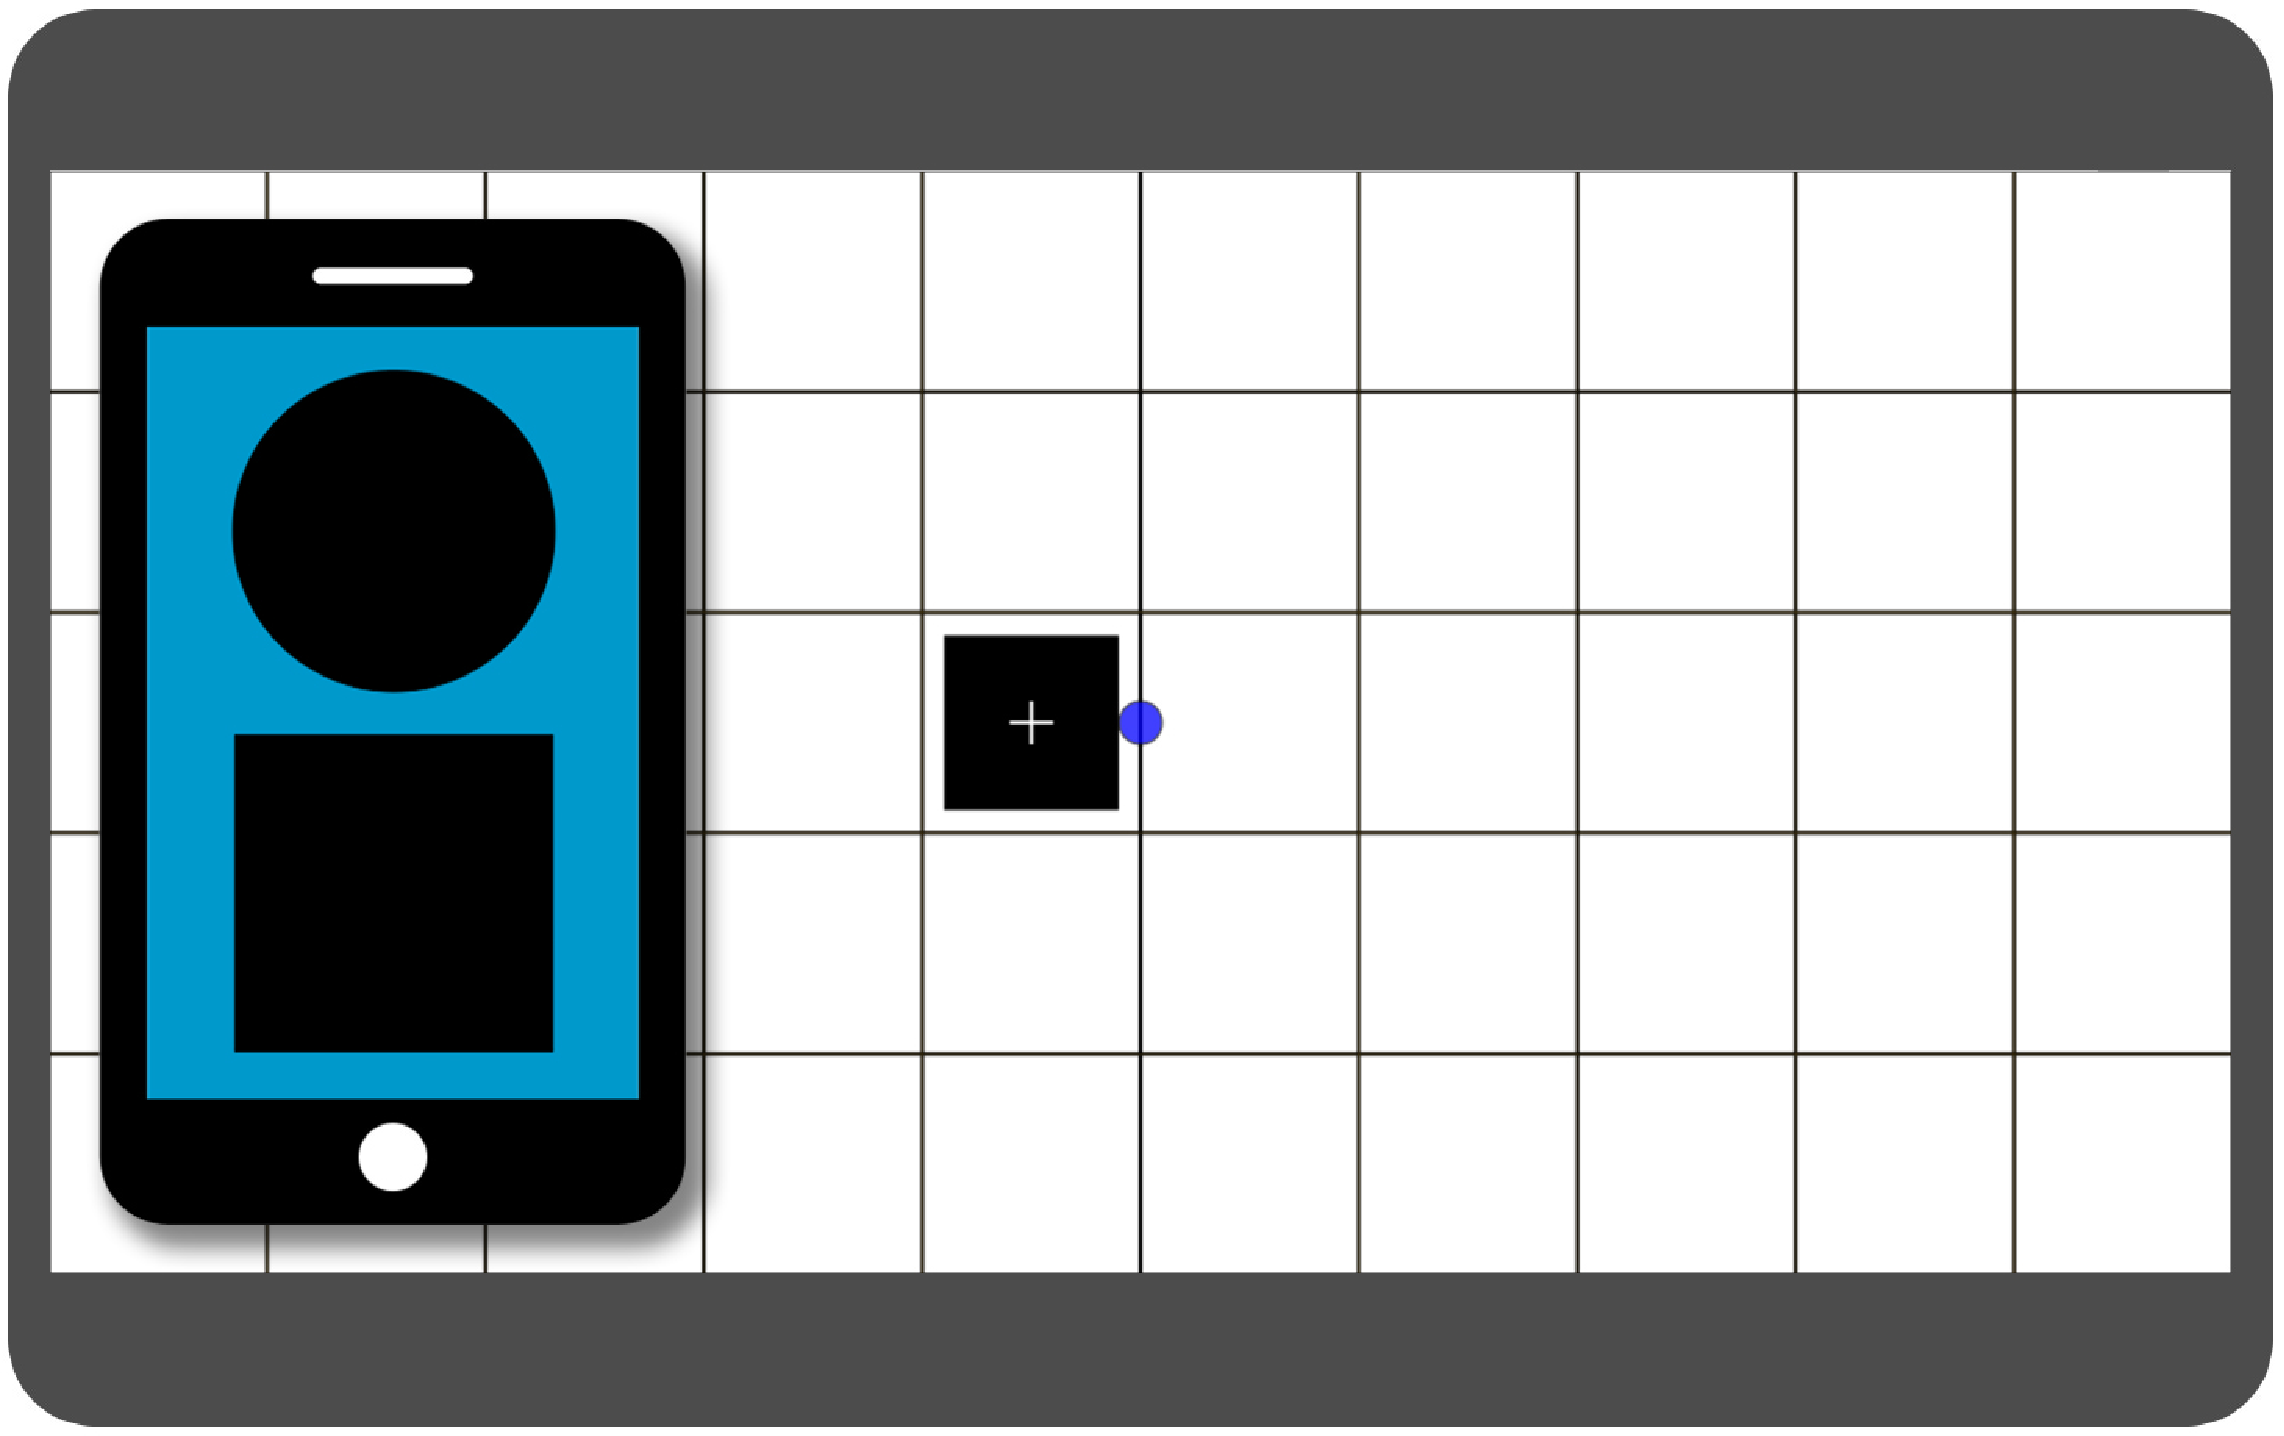
\includegraphics[width = 0.48\columnwidth]{images/pushScreen.pdf}\label{fig:pushScreen}}
	\hspace{0.01\columnwidth}
	\subfloat[\pull]{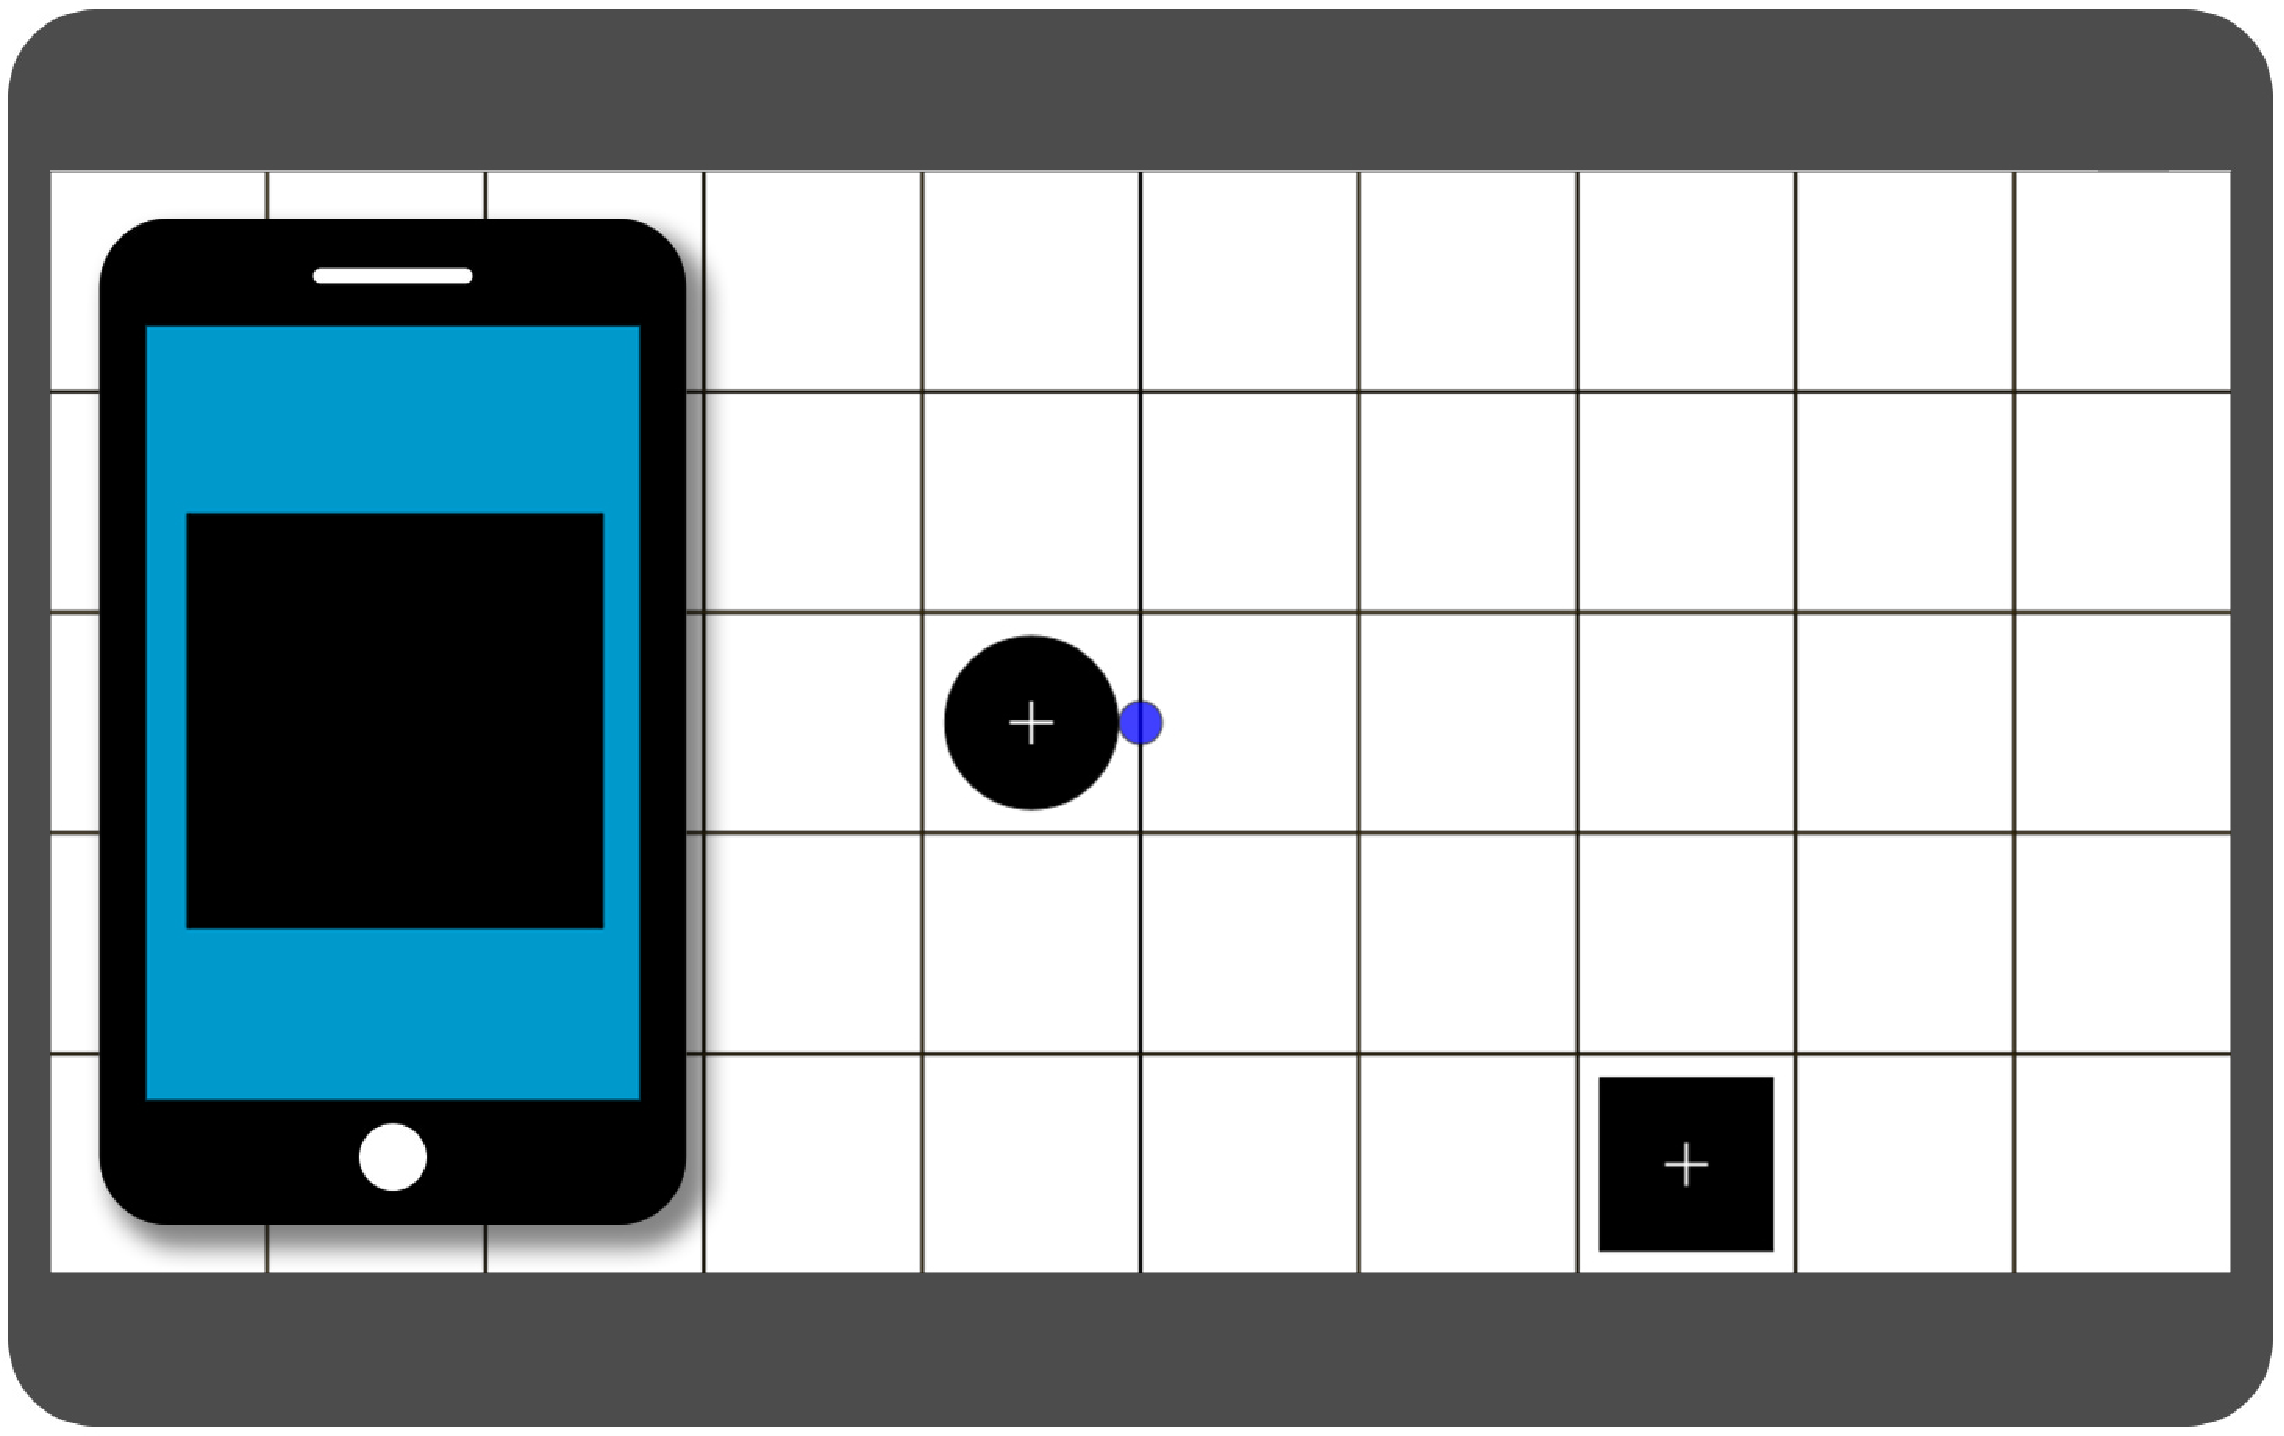
\includegraphics[width = 0.48\columnwidth]{images/pullScreen.pdf}\label{fig:pullScreen}}
	\end{minipage}
	\caption{The screens on both the large display and the phone for the \accuracy.}
\end{figure}

During the \push phase of each experiment, users would be presented with one shape on the screen and two on the smartphone, as seen in \cref{fig:pushScreen}.
Here, the screen would tell the users what the correct shape was, and the user had to perform the correct gesture by selecting the correct shape on the phone.
During the \pull phase of the experiment, users would be presented with two shapes on the large screen, and one shape on the smart phone.
Here, the phone would be telling users what the correct shape was and users would have to grab the correct shape from the large display. 
Within the experiment, we conducted two separate studies, using the same implementation of techniques and experimental method. 

\subsubsection{Study One: The Target Experiment} 
During the \target, The pointing circle was solid blue, 
There was also a bright yellow highlight in whichever cell the pointer was currently over.
This can be seen in \Cref{fig:target}.
This was for providing feedback to the user about whether or not he was hitting the correct cell. 

\subsubsection{Study Two: The Accuracy Experiment}
During the \accuracy, we added a white cross to each target to provide a precise point for the users to hit.
The pointing circle was also made opaque so that users could better see the cross, as well as removing the highlight so that users would not feel that hitting any location on the cell was acceptable.
This can be seen in \Cref{fig:accuracy}.
In study two, we explicitly asked users to be as precise as possible while performing each technique.

\begin{figure}[H]
\centering
\subfloat[]{\includegraphics[width = 0.13\columnwidth]{images/target.pdf}\label{fig:target}}
\hspace{0.05\columnwidth}
\subfloat[]{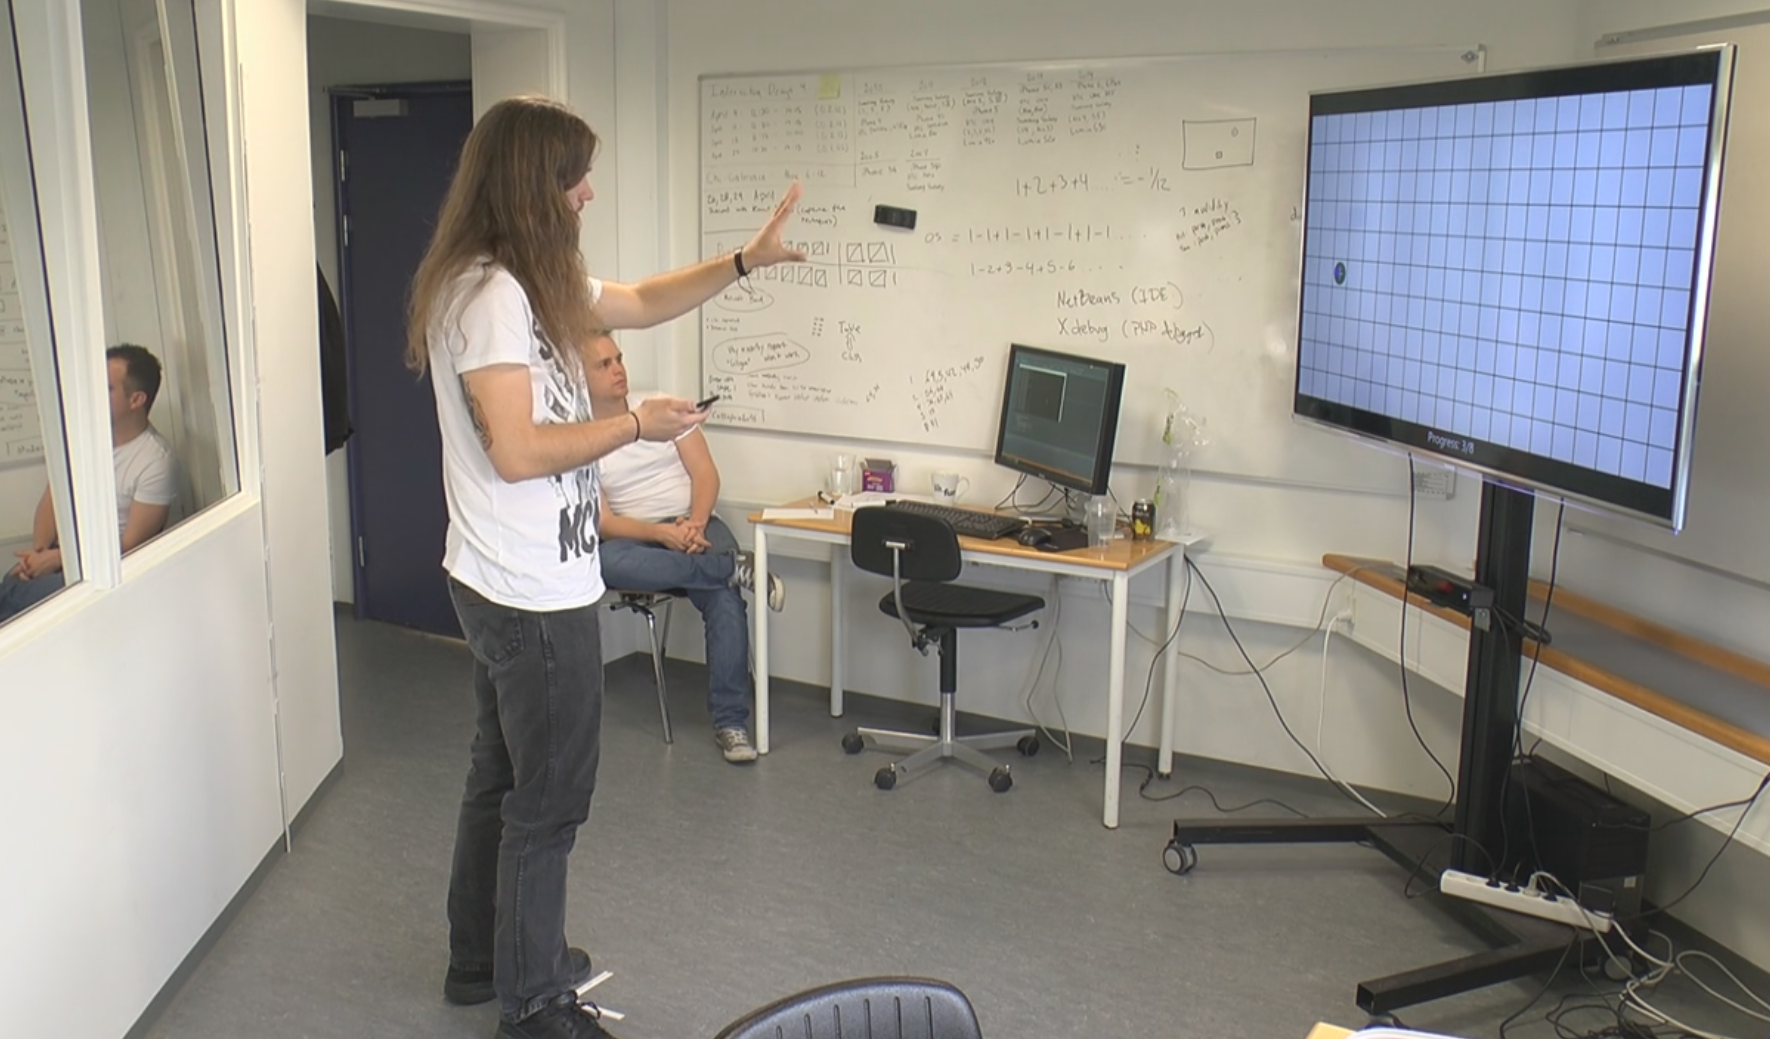
\includegraphics[width = 0.13\columnwidth]{images/accuracy.pdf}\label{fig:accuracy}}
\caption{\protect\subref{fig:target} The targets in the first part of the experiment. \protect\subref{fig:accuracy} The targets in the second part of the experiment.}
\end{figure}

\subsection{Experimental Setup} \label{sec:setup}
% The setup and the hardware used in the experiment
The experiment was conducted in laboratory setting where we setup a large 65'' screen (1920$\times$1080 pixels) and a smaller 42'' screen (1024$\times$768 pixels) as seen in \Cref{fig:setupPhoto}.
A Microsoft Kinect v2 was mounted below the large display (81 cm above the floor) and we marked the floor with a cross (200 cm from the Kinect) where participants were instructed to stand on.
We chose 200 cm from the display because this is an optimal operating distance for the Kinect.
The height of the Kinect with regards to the floor was chosen through physical adjustment to get the optimal position for a person who is 180 cm tall, given that the average height of Danish men is 183 cm, and women is 169 cm. 
The phone we used in this experiment was a Samsung Galaxy S2 (4.3'' screen).
The setup is illustrated in \Cref{fig:setup}.

\begin{figure}[H]
\subfloat[]{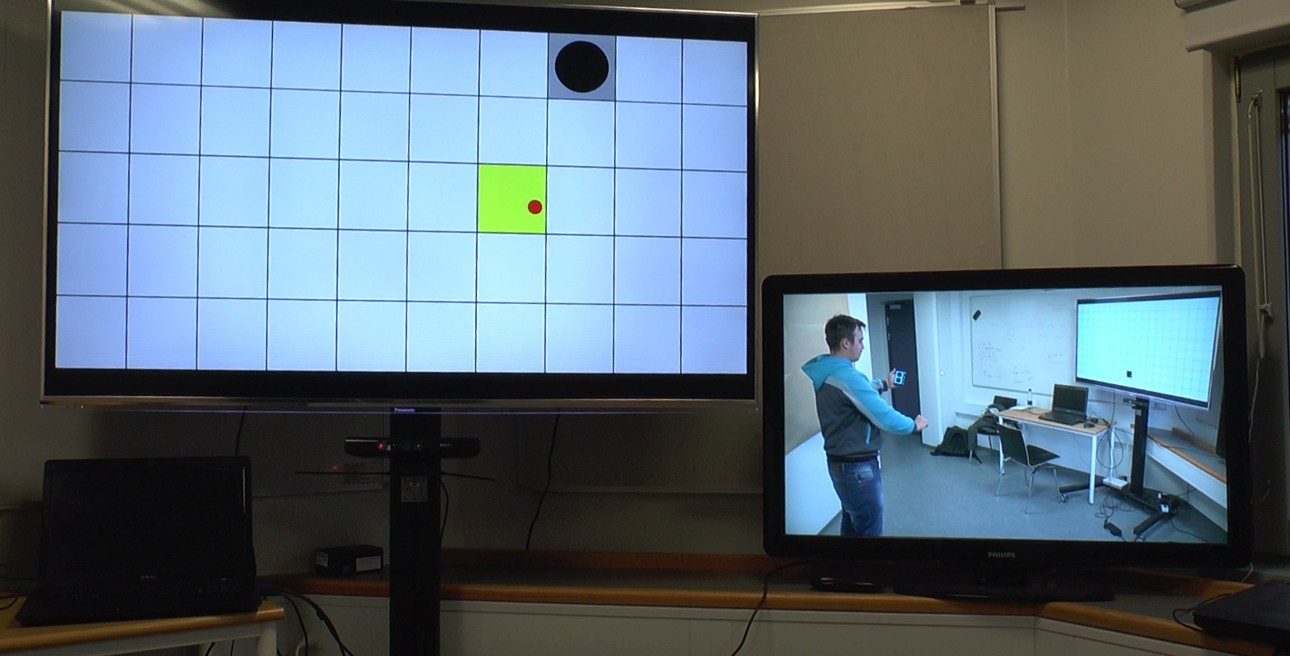
\includegraphics[width = 0.6\columnwidth]{images/setup.jpg}\label{fig:setupPhoto}}
\subfloat[]{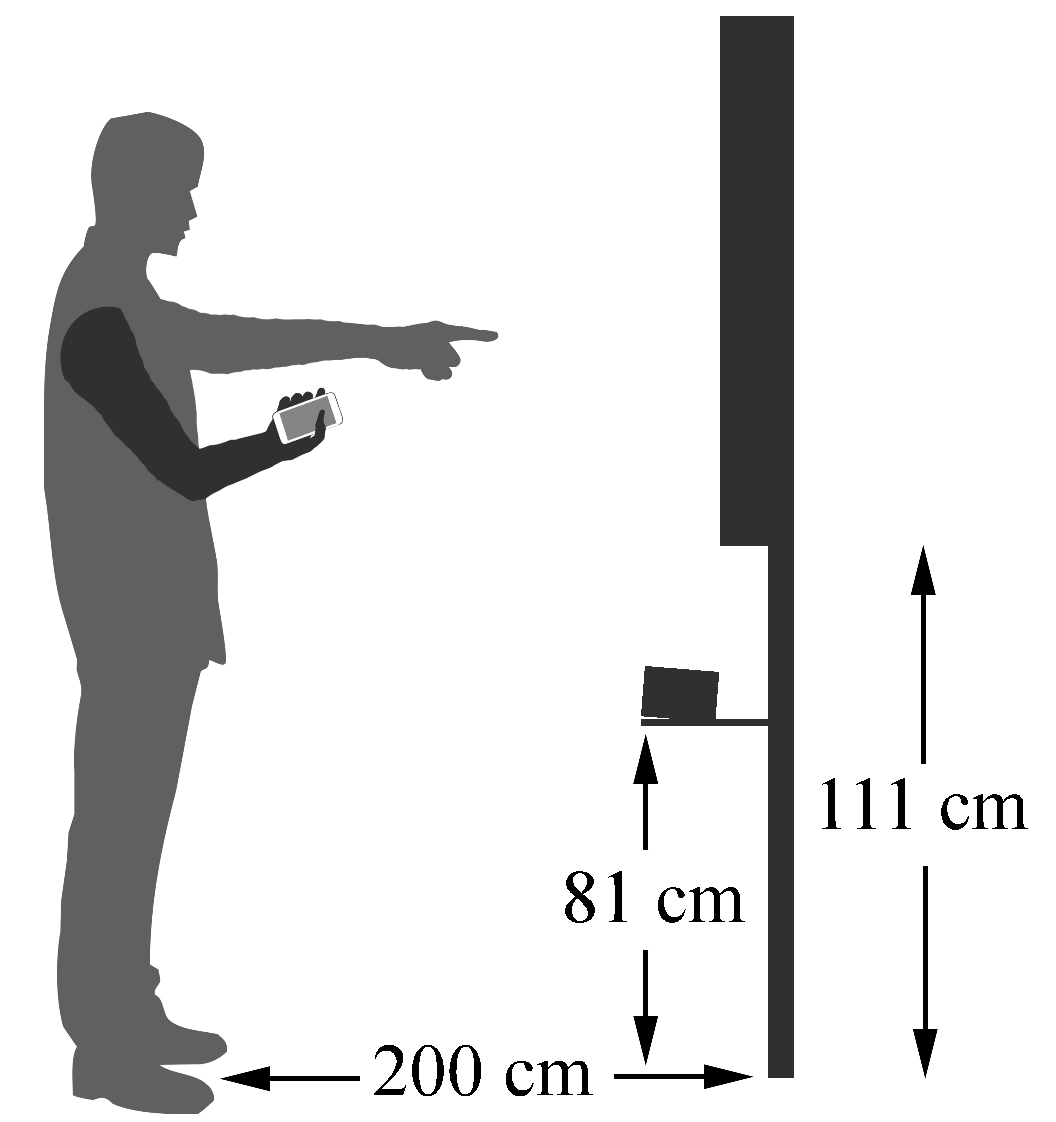
\includegraphics[width = 0.37\columnwidth]{images/setup.pdf}\label{fig:setup}}
\caption{\protect\subref{fig:setupPhoto} the setup in the usability lab. \protect\subref{fig:setup} illustrates the setup and distance between participant and screen, floor and Kinect, and floor and the bottom of the large display.}
\end{figure}

\subsubsection{Experimental Design} \label{}
% (explain practice targets, targets, grid, before procedure and task section)
% Also, explain sequences and the different distances between targets
A within-group design was used for the experiment and each participant used all 8 techniques once during the experiment.
We have 2 different target sizes (large, small) and 8 techniques (push = 4, pull = 4) as the independent variables.
For each technique there are a total of 18 targets and 3 practice targets at the beginning of each technique. 
Practice targets allow the participants to get familiar with the technique before we start collecting data for a technique.
The order in which the participants are presented with a technique is randomized to minimize the learning effect of each technique.
For both \studyone: \target and \studytwo: \accuracy 51\% of the participants started with \push techniques and 49\% started with \pull techniques.
For \studyone 27\% of the participants started the test with \grab, 21\% with \swipe, 25\% with \throw, and 27\% with \tilt.
Similarly, for \studytwo 22\% of the participants started the test with \grab, 27\% with \swipe, 24\% with \throw, and 27\% with \tilt.
For \studyone the total amount of attempts collected were 2 target sizes $\times$ 8 techniques $\times$ 9 repetitions $\times$ 51 participants = 7344 attempts and for \studytwo the total is 2 target sizes $\times$ 8 techniques $\times$ 9 repetitions $\times$ 33 participants = 4752 attempts.

\subsubsection{Participants}
For the \studyone: \target, 51 people took part in the experiment. They ranged in age from 21 to 52 (M: 27,98) and were between 1.56m and 1.98m (M: 1,79m). 
15.7\% of participants were women, and 84.3\% were male.
All of the participants owned smartphones and had owned one for 2-12 years (M:5.9).

For the \studytwo: \accuracy, 33 people took part. They were anywhere between 20 and 55 years old (M: 23.18) and were between 1.56m and 2m tall (M: 1.77m).
30.3\% of the participants were female, while 69.7\% were male.
They had all owned smartphones between 1 and 9 years (M: 5.5).

\subsubsection{Task \& Procedure} \label{sec:procedure}
The task and procedure were the same for both studies, with the additional instructions in \studytwo to be as precise as possible.
Before a participant starts the experiment, the general purpose of the study is explained to the participant and we inform them about what is going to happen.
Then a demonstration video of a technique is shown on the large screen and after watching the video it plays in a loop on the small screen.
The participant is then presented with the grid and one target after another will appear in the grid until the participant has attempted to hit all targets.
After completing one technique the remaining techniques follow with the same procedure as the first until all 8 techniques have been performed.
When a participant has done all the techniques we give them a short demographic questionnaire including age, height, gender, current phone, year of first smartphone, and if they have had prior experience with systems like the Nintendo Wii or the Microsoft Kinect.
The average time for completing the experiment per participant was 25$\pm$5 minutes. 